% 
% Резюме на основе стиля moderncv
%



\documentclass[11pt,a4paper,sans]{moderncv}        % possible options include font size ('10pt', '11pt' and '12pt'), paper size ('a4paper', 'letterpaper', 'a5paper', 'legalpaper', 'executivepaper' and 'landscape') and font family ('sans' and 'roman')

% moderncv themes
\moderncvstyle{casual}                             % style options are 'casual' (default), 'classic', 'banking', 'oldstyle' and 'fancy'
\moderncvcolor{blue}                           % color options 'black', 'blue' (default), 'burgundy', 'green', 'grey', 'orange', 'purple' and 'red'
%\renewcommand{\familydefault}{\sfdefault}         % to set the default font; use '\sfdefault' for the default sans serif font, '\rmdefault' for the default roman one, or any tex font name
%\nopagenumbers{}                                  % uncomment to suppress automatic page numbering for CVs longer than one page

% character encoding
\usepackage[utf8]{inputenc}

% Для QuickStart
\usepackage{tikz,pgfplots,pgfplotstable}
%\pgfplotsset{width=8cm,compat=1.8}

% Резюме по-русски
%\usepackage[english, russian]{babel}
% Резюме по-английски
\usepackage[russian, english]{babel}

% FIXME: проблемы с генерацией pdf на русском языке, какие-то шрифты не гененрируются или не установлены
%\usepackage[T2A]{fontenc}

% adjust the page margins
\usepackage[scale=0.75]{geometry}
%\setlength{\hintscolumnwidth}{3cm}                % if you want to change the width of the column with the dates
%\setlength{\makecvtitlenamewidth}{10cm}           % for the 'classic' style, if you want to force the width allocated to your name and avoid line breaks. be careful though, the length is normally calculated to avoid any overlap with your personal info; use this at your own typographical risks...


%
% Перевод часто используемых словосочетаний
%
\makeatletter
\newcommand{\newlanguagecommand}[1]{%
  \newcommand#1{%
    \@ifundefined{\string#1\languagename}
      {``No def of \texttt{\string#1} for \languagename''}
      {\@nameuse{\string#1\languagename}}%
  }%
}
\newcommand{\addtolanguagecommand}[3]{%
  \@namedef{\string#1#2}{#3}}
\makeatother

%
%
%
\newlanguagecommand{\myname}
\addtolanguagecommand{\myname}{english}{Sergey}
\addtolanguagecommand{\myname}{russian}{Сергей}

\newlanguagecommand{\mysurname}
\addtolanguagecommand{\mysurname}{english}{Kryazhevskikh}
\addtolanguagecommand{\mysurname}{russian}{Кряжевских}

%
% Города
%
\newlanguagecommand{\cityspb}
\addtolanguagecommand{\cityspb}{english}{St. Petersburg (remotelly)}
\addtolanguagecommand{\cityspb}{russian}{Санк-Петербург (удалённо)}

\newlanguagecommand{\citymoscow}
\addtolanguagecommand{\citymoscow}{english}{Moscow (remotelly)}
\addtolanguagecommand{\citymoscow}{russian}{Москва (удалённо)}

\newlanguagecommand{\cityperm}
\addtolanguagecommand{\cityperm}{english}{Perm}
\addtolanguagecommand{\cityperm}{russian}{Пермь}

\newlanguagecommand{\citykirov}
\addtolanguagecommand{\citykirov}{english}{Kirov}
\addtolanguagecommand{\citykirov}{russian}{Киров}

%
% Страны
%
\newlanguagecommand{\country}
\addtolanguagecommand{\country}{english}{Russia}
\addtolanguagecommand{\country}{russian}{Россия}

%
%
%
\newlanguagecommand{\achievements}
\addtolanguagecommand{\achievements}{english}{Detailed achievements}
\addtolanguagecommand{\achievements}{russian}{Основные достижения}

%
% Места работы
%
\newlanguagecommand{\ors}
\addtolanguagecommand{\ors}{english}{<<Otdelenie Razrabotki System>> JSC}
\addtolanguagecommand{\ors}{russian}{ОАО <<Отделение Разработки Систем>>}

\newlanguagecommand{\simos}
\addtolanguagecommand{\simos}{english}{Scientific and Technical Center <<SIMOS>> CJSC}
\addtolanguagecommand{\simos}{russian}{ЗАО <<НТЦ Симос>>}

\newlanguagecommand{\permenergo}
\addtolanguagecommand{\permenergo}{english}{<<Permenergo>> JSC}
\addtolanguagecommand{\permenergo}{russian}{ОАО <<Пермэнерго>>}

\newlanguagecommand{\gorkilibrary}
\addtolanguagecommand{\gorkilibrary}{english}{Regional Multipurpose Library named after Maxim Gorky}
\addtolanguagecommand{\gorkilibrary}{russian}{Краевая универсальная библиотека им. А.М. Горького}


\newlanguagecommand{\ertelecom}
\addtolanguagecommand{\ertelecom}{english}{<<ER-Telecom Holding>> JSC}
\addtolanguagecommand{\ertelecom}{russian}{АО <<ЭР-Телеком Холдинг>>}

\newlanguagecommand{\prognoz}
\addtolanguagecommand{\prognoz}{english}{<<Prognoz>> CJSC}
\addtolanguagecommand{\prognoz}{russian}{ЗАО <<Прогноз>>}

\newlanguagecommand{\proitr}
\addtolanguagecommand{\proitr}{english}{<<Pro IT>> LLC}
\addtolanguagecommand{\proitr}{russian}{ООО <<Про Ай-Ти Ресурс>>}

\newlanguagecommand{\ibs}
\addtolanguagecommand{\ibs}{english}{<<IBS>> LLC}
\addtolanguagecommand{\ibs}{russian}{ООО ИБС-Пермь, <<Группа компаний IBS>>}

\newlanguagecommand{\simpl}
\addtolanguagecommand{\simpl}{english}{<<PIT>> LLC}
\addtolanguagecommand{\simpl}{russian}{ООО ПИТ, <<Группа компаний Simpl>>}

\newlanguagecommand{\bia}
\addtolanguagecommand{\bia}{english}{<<BIA Technologies>> LLC}
\addtolanguagecommand{\bia}{russian}{ООО <<БиАйЭй Технолождиз>>}


%
% Должности
%
\newlanguagecommand{\seniorbigdata}
\addtolanguagecommand{\seniorbigdata}{english}{Senior BigData Engineer}
\addtolanguagecommand{\seniorbigdata}{russian}{Инженер больших данных}

\newlanguagecommand{\sysarchitect}
\addtolanguagecommand{\sysarchitect}{english}{System Architect}
\addtolanguagecommand{\sysarchitect}{russian}{Системный архитектор}


\newlanguagecommand{\chiefsoftdeveloper}
\addtolanguagecommand{\chiefsoftdeveloper}{english}{Chief Software Developer}
\addtolanguagecommand{\chiefsoftdeveloper}{russian}{Главный разработчик}

\newlanguagecommand{\leadsoftdeveloper}
\addtolanguagecommand{\leadsoftdeveloper}{english}{Leading Software Developer}
\addtolanguagecommand{\leadsoftdeveloper}{russian}{Ведущий разработчик}

\newlanguagecommand{\seniorcondeveloper}
\addtolanguagecommand{\seniorcondeveloper}{english}{Senior Consultant and Software Developer}
\addtolanguagecommand{\seniorcondeveloper}{russian}{Старший консультант-разработчик}

\newlanguagecommand{\designengineer}
\addtolanguagecommand{\designengineer}{english}{Design Engineer in Electronics}
\addtolanguagecommand{\designengineer}{russian}{Инженер-конструктор}

\newlanguagecommand{\leadscientist}
\addtolanguagecommand{\leadscientist}{english}{Senior Scientist}
\addtolanguagecommand{\leadscientist}{russian}{Старший научный сотрудник}

\newlanguagecommand{\leadsysadmin}
\addtolanguagecommand{\leadsysadmin}{english}{Leading System Engineer}
\addtolanguagecommand{\leadsysadmin}{russian}{Ведущий инженер}

\newlanguagecommand{\seniordba}
\addtolanguagecommand{\seniordba}{english}{Senior Database Administrator}
\addtolanguagecommand{\seniordba}{russian}{Руководитель направления баз данных}



% personal data
\name{\myname}{\mysurname}

\iflanguage{russian}
{\title{Системная Архитектура и Программирование}}
{\title{System Architect and Software Engineer}}


%
\address{\cityperm}{\country}
%
% the optional "type" of the phone can be "mobile" (default), "fixed" or "fax"
\phone[mobile]{+7~922~324~10~10}
%%\phone[fixed]{+2~(345)~678~901}
%%\phone[fax]{+3~(456)~789~012}
\email{soliverr@gmail.com}
%%\homepage{www.johndoe.com}
\social[linkedin]{sergey-kryazhevskikh-8128b2108}
%%\social[twitter]{jdoe}
\social[github]{soliverr}
\social[gitlab]{soliverr}
\photo[64pt][0.4pt]{photo.jpeg}
\iflanguage{russian}
{\quote{Инженер больших данных. Системный архитектор. Инженер DevOps. Системный и прикладной программист. Инженер-исследователь. Разработчик и администратор баз данных}}
{\quote{BigData Engineer. System Architect. DevOps. Software Developer. Research Engineer. DataBase Administrator.}}

\begin{document}
%-----       resume       ---------------------------------------------------------
\makecvtitle

\iflanguage{russian}{\section{Обзор профессиональных навыков}}{\section{<<Quick start>> CV review}}

\pgfplotstableread{ % data 
	Label                            Programming DevOps    DBA      Architect
	{R\&D epoch (1995-2004)}         40          25        10       25
	{SysAdmin epoch (2005 - 2007)}   15          45        20       20
	{DataBase epoch (2007 - 2018)}   15          25        50       10
	{BigData epoch (2019 - current)} 45          25        5        25	
}\overviewdata

\begin{center}
\begin{tikzpicture}

\begin{axis}[
xbar stacked,   % Stacked horizontal bars
xmin=0,         % Start x axis at 0
ytick=data,     % Use as many tick labels as y coordinates
xtick style={draw=none},
ytick style={draw=none},
%enlarge y limits=0.8,
legend style={
	at={(1.05,0.05)},
	%at={(axis cs:65,0.2)},
	anchor=south west,
	%draw=none,
},
yticklabels from table={\overviewdata}{Label}  % Get the labels from the Label column of the \datatable
]
\addplot [fill=green!50] table [x=Programming, meta=Label,y expr=\coordindex] {\overviewdata};
\addplot [fill=blue!20] table [x=DevOps, meta=Label,y expr=\coordindex] {\overviewdata};
\addplot [fill=orange!50] table [x=DBA, meta=Label,y expr=\coordindex] {\overviewdata};
\addplot [fill=red!40] table [x=Architect, meta=Label,y expr=\coordindex] {\overviewdata};
\legend{Programming,DevOps,DBA,Architect}
\end{axis}
\end{tikzpicture}
\end{center}


%\iflanguage{russian}
%{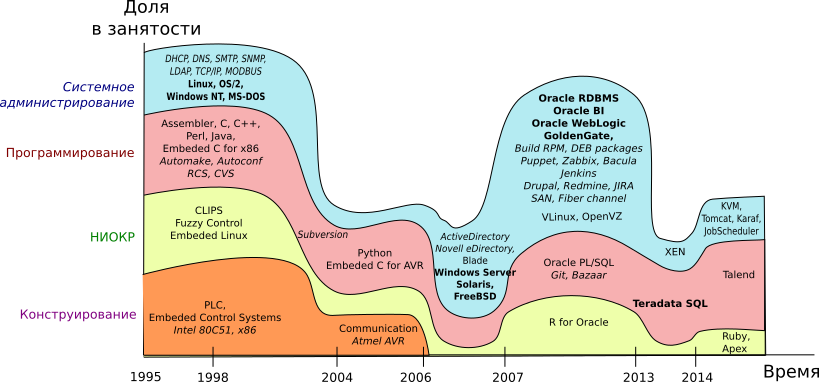
\includegraphics[width=0.85\linewidth]{resume_ru.png}}
%{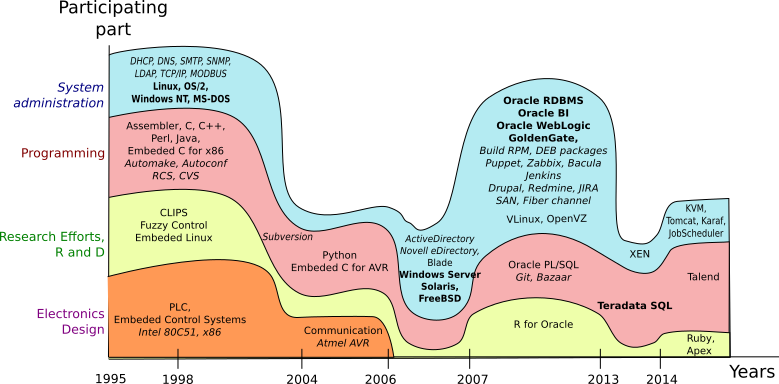
\includegraphics[width=0.90\linewidth]{resume_en.png}}

\iflanguage{russian}{\section{Сертификаты}}{\section{Certification}}

\cvitem{Scala}{Scala-ReactiveX: Programming Reactive Systems: 2021}
\cvitem{BigData}{Yandex Big Data Specialization:\newline{}
	Big Data Applications: Real-Time Streaming: 2020\newline{}
	Big Data Applications: Machine Learning at Scale: 2019\newline{}
	Big Data Analysis: Hive, Spark SQL, DataFrames and GraphFrames: 2019\newline{}
	Big Data Essentials: HDFS, MapReduce and Spark RDD: 2019
}
\cvitem{OCP}{Oracle Certified Professional: 2015 -- 11g, 2012 -- 9g}
\cvitem{OCA}{Oracle Certified Associate: 2008 -- 9i}
\cvitem{Linux}{Novell Certified Linux Administrator: 2010,\newline{}Linux Professional Institute, LPI-I: 2008}{}{}

\newpage

\iflanguage{russian}{\section{Образование}}{\section{Education}}

\iflanguage{russian}
{\cventry{1995--1998}{Инженер-исследователь}{{\protect\httplink[Вятский Государственный Университет]{www.vyatsu.ru}}}{Киров}{\textit{Высшее специальное}}{Окончил аспирантуру по специальности "Системы автоматического управления"}}
{\cventry{1995--1998}{Research Engineer}{{\protect\httplink[Vyatka State University]{www.vyatsu.ru}}}{Kirov}{\textit{Higher professional}}{Postgraduated study in "Automatic control systems"}}

\iflanguage{russian}
{\cventry{1990--1995}{Инженер}{{\protect\httplink[Вятский Государственный Университет]{www.vyatsu.ru}}}{Киров}{\textit{Высшее}}{Диплом с отличием по специальности "Инженер---электроник-конструктор-технолог электронно-вычислительных средств"}}
{\cventry{1990--1995}{Engineer}{{\protect\httplink[Vyatka State University]{www.vyatsu.ru}}}{Kirov}{\textit{Higher}}{Diploma with honors in "Electronic-Constructor-Technologist Engineer of electronic computing systems"}}


\iflanguage{russian}{\section{Опыт работы}}{\section{Experience}}

%
% Шаблон для заполнения
%
% \cventry{year--year}{Degree}{Institution}{City}{\textit{Grade}}{Description}  % arguments 3 to 6 can be left empty
%
%\cventry{2017--2018}{\seniorcondeveloper}
%{\protect\httplink[\ibs]{ibs.ru}}
%{\citymoscow, \country}
%{}
%{\iflanguage{russian}
%	{Краткое описание не более 1--2 строк}{General description no longer than 1--2 lines.}\newline{}
%	\achievements:
%	\begin{itemize}
%		\item \iflanguage{russian}{ИТ Архитектура}{IT Architecture}
%		\begin{itemize}
%			\item \iflanguage{russian}{Один}{One}
%			\item \iflanguage{russian}{Два}{Two}
%		\end{itemize}
%		\item \iflanguage{russian}{Разработка программного обеспечения}{Software development}
%		\begin{itemize}
%			\item \iflanguage{russian}{Один}{One}
%			\item \iflanguage{russian}{Два}{Two}
%		\end{itemize}
%		\item \iflanguage{russian}{Администрирование баз данных Oracle}{Oracle DBA}
%		\begin{itemize}
%			\item \iflanguage{russian}{Один}{One}
%      \item \iflanguage{russian}{Два}{Two}
%		\end{itemize}
%		\item \iflanguage{russian}{DevOps и системное администрирование}{DevOps and System administration}
%		\begin{itemize}
%			\item \iflanguage{russian}{Один}{One}
%			\item \iflanguage{russian}{Два}{Two}
%		\end{itemize}
%	\end{itemize}
%}
%


%
% Последние 3 места работы. Актуальные навыки 
%
\iflanguage{russian}{\subsection{Актуальные навыки}}{\subsection{Actual valid skills}}

\cventry{2020--current}{\seniorbigdata}
{\protect\httplink[\bia]{bia-tech.ru}}
{\cityspb, \country}
{}
{\iflanguage{russian}
	{Системная архитектура, внедрение и сопровождение сервисов в кластере на базе Hadoop. Разработка прикладного программного обеспечения для вычислительного кластера с использованием Spark, Kafka и др.}
	{Design, deploy and maintain on-premise Hadoop based cluster. Development business software
	applications used Spark, Kafka and more.}
	\newline{}
	\achievements:
	\begin{itemize}
		\item \iflanguage{russian}{Техническое лидерство}{Technical Leader}
		\begin{itemize}
			\item \iflanguage{russian}
				{Популяризация широкого спектра отрытых технологий в компании: проведение семинаров и обучающих курсов}
				{Popularization of a wide range of open-source technologies in the company: holding seminars and training courses }
			\item \iflanguage{russian}
				{Ведение дипломных проектов студентов}
				{Conducting graduation projects of students}
			\item \iflanguage{russian}
				{Ведение технической документации}
				{Writing wikies and technical documentation: Sphinx-doc}
		\end{itemize}
		\item \iflanguage{russian}{ИТ Архитектура}{IT Architecture}
		\begin{itemize}
			\item \iflanguage{russian}
				{Разработка системной архитектуры подсистем озера данных на базе Hadoop}
				{System architecture desing of Hadoop based DataLake}
			\item \iflanguage{russian}
				{Разработка механизма миграции озера данных в дом данных}
				{Migration data storage paradigm: from DataWareHouse and DataLake to LakeHouse }
			\item \iflanguage{russian}
				{Разработка и внедрение архитектуры потоковой обработки данных с использованием Kafka, Debezium, Spark Structured Streaming, Delta-tables}
				{Desing and implementation of streaming processing subsystem: Kafka, Debezium, Spark Structured Streaming, Delta-tables}
			\item \iflanguage{russian}
				{Разработка и внедренеие архитекутуры обработки данных в кластере Hadoop: Airflow, Celery, DASK}
				{Desing and implementation of a data ingestion subsystem: Airflow, Celery, DASK}
			\item \iflanguage{russian}
				{Разработка архитектуры интеграции Hadoop и Kubernetes}
				{Hadoop and Kubernetes integration}
			\item \iflanguage{russian}
				{Разработка архитектуры DataGovernance и DataLineage: LinkedIn DataHub, Atlas}
				{Desing and implementation of a data governance and data lineage subsystem: LinkedIn DataHub, Apache Atlas}
			\item \iflanguage{russian}
				{Разработка архитектуры подсистемы качества данных: GreatExpectaion, Apache Griffin}
				{Design and implementation of a data quality and data assurance subsystem: Great Expectations, Apache Griffin}
			\item \iflanguage{russian}
				{Разработка архитектуры виртуализации данных и интеграции озера данных с существующим хранилищем данных, миграция с Hive на Trino}
				{Desing and implementation of data virtualization subsystem: Trino; DWH intergation: PolyBase}
			\item \iflanguage{russian}
				{Разработка и внедрение архитектуры оркестрации данных с использованием Alluxio}
				{Desing of data orchestration subsystem: Alluxio }
		\end{itemize}
		\item \iflanguage{russian}{Разработка программного обеспечения}{Software development}
		\begin{itemize}
			\item \iflanguage{russian}
				{Разработка коннекторов Kafka потоковой обработки на Scala и Python}
				{Developing of Kafka connectors on Scala and Python}
			\item \iflanguage{russian}
				{Реализация табличной модели хранения на базе Delta-таблиц (delta.io)}
				{Developing of streaming storage table model based on Delta-tables (delta.io) on Scala}
			\item \iflanguage{russian}
				{Разработка модулей построения DAG для Airflow}
				{Developing DAG factory and DAGs for Airflow}
			\item \iflanguage{russian}
				{Разработка прототипов моделей данных для обработки данных в реальном времени на Python с использованием Pandas, DASK, pySpark}
				{Developing buisiness models for realtime data processing using Pandas, DASK, pySpark}
		\end{itemize}
		\item \iflanguage{russian}{Администрирование баз данных}{Data Bases}
		\begin{itemize}
			\item \iflanguage{russian}
				{Участие в проектах для MS SQL Server}
				{Participation in projects for MS SQL Server}
      		\item \iflanguage{russian}
      			{Внедрение и сопровождение СУБД PostgreSQL в кластерном режиме, интеграция с Hadoop с использованием KafkaConnect и Debezium}
      			{Integration cluster PostgreSQL with Hadoop: Patroni}
		\end{itemize}
		\item \iflanguage{russian}{DevOps и системное администрирование}{DevOps and System administration}
		\begin{itemize}
			\item \iflanguage{russian}
				{Сопровождение собственного кластера Hadoop: распределение ресурсов, организация отказоустойчивости, организация резервного копирования}
				{Maintain on-premise Hadoop clusters}
			\item \iflanguage{russian}
				{Внедренеие системы сопровождения кластера Hadoop с использование Ansible и GitLab}
				{Implement DevOps techniques to support Hadoop clusters: Ansible, GitLab}
			\item \iflanguage{russian}
				{Создание собственных ролей Ansible для сопровождения кластера Hadoop}
				{Developing own Annible roles, Ansible and GitLab integration}
			\item \iflanguage{russian}
				{Миграция производственного кластера с Hortownworks Data Platform на ванильные дистрибутивы кластерного ПО, проработка методологии обновления калстерного ПО}
				{Migration of production Hadoop cluster from Hortonworks Data Platform to vanilla Hadoop}
			\item \iflanguage{russian}
				{Интеграция Hadoop и Docker Swarm с использованием Portainer}
				{Docker Swarm and Hadoop integration: Portainer}
			\item \iflanguage{russian}
				{Внедрение системы мониторинга: с использованием Prometheus/Grafana/AlertManager, ElasticSearch/Filebeat/Kibana}
				{Implementation of monitoring system for Kafka and Hadoop: Prometheeus, Grafana, AlertManager, ElasticSearch, Filebeat, Kibana}
		\end{itemize}
	\end{itemize}
}

\cventry{2018--2020}{\chiefsoftdeveloper}
{\protect\httplink[\simpl]{simpl-group.ru}}
{\cityspb, \country}
{}
{\iflanguage{russian}
	{Управление процессом разработки, разработка архитектуры, разработка прикладного программного обеспечения, внедрение программно-аппаратного комплекса разработанного решения для проекта в нефтегазовой отрасли}
	{Process management, architecture design, software development in one gas and oil industry project}
	\newline{}
	\achievements:
	\begin{itemize}
		\item \iflanguage{russian}{Тимлид}{Technical Leader}
		\begin{itemize}
			\item \iflanguage{russian}
				{Управление и организация работы команды разработчиков: 5-12 человек}
				{Technical leading and small team management: 5-12 developers}
			\item \iflanguage{russian}
				{Выбор системы ведения проекта: Jira, Trello, Ora.pm}
				{Project management with Jira, Trello, Ora.pm}
			\item \iflanguage{russian}
				{Внедрение Scrumban в управление проектом: Ora.pm}
				{Scumban implementation}
			\item \iflanguage{russian}
				{Внедрение Scrum Poker в планирование спринтов}
				{Scrum Pocker implementation}
			\item \iflanguage{russian}
				{Поддержание духа startup в команде разработчиков}
				{Endorse team startup spirit}
			\item \iflanguage{russian}
				{Внедрение системы планирования спринтов на основе общей оценки скорости работы команды и индивидуальной скорости работы разработчика. Индекс активности разработчика. Автоматизация планирования с использованием MSProject, GanttProject, TaskJuggler}
				{Project planning: MSProject, GanttProject, TaskJuggler}
			\item \iflanguage{russian}
				{Внедрение методологии управления релизами, организация выходного тестирования поставляемых заказчику решений в среде UAT}
				{Implement test-based release management aproach}
		\end{itemize}
		\item \iflanguage{russian}{ИТ Архитектура}{IT Architecture}
		\begin{itemize}
			\item \iflanguage{russian}
				{Разработана архитектура вычислительного кластера на базе стека технологий BigData: Hadoop HDFS/YARN, ZooKeeper, Spark, Hive, Kyuubi Thrift JDBS/ODBC Server, Alluxio}
				{Desing and implementation of Hadoop-based calculation cluster: Hadoop HDFS/YARN, ZooKeeper, Spark, Hive, Kyuubi Thrift JDBS/ODBC Server, Alluxio}
			\item \iflanguage{russian}
				{Проработка целевой архитектуры распределённой вычислительной системы с использованием различных стеков технологий}
				{Architecture desing for a distributed calculation subsystem to migrate from Oracle Model}
			\item \iflanguage{russian}
				{Проработка архитектуры прикладного программного обеспечения и взаимодействия компонент разрабатываемого решения}
				{System architecture desing for all software components of the projects}
			\item \iflanguage{russian}
				{Участие в технических совещаниях с заказчиком, участие в защите решения у заказчика, написание технической документации}
				{Participation in technical meetings with customers, writing technical documentation}
		\end{itemize}
		\item \iflanguage{russian}{Разработка программного обеспечения}{Software Development}
		\begin{itemize}
			\item \iflanguage{russian}
				{Ведение задач в Ora.pm. Миграция системы планирования из Jira}
				{Planning in Jira, modev to Ora.pm}
			\item \iflanguage{russian}
				{Разработка моделей данных и PL/SQL кода для интеграци существующей системы с распределённым вычислительным кластером: Oracle PL/SQL}
				{Writing Oracle PL/SQL packages}
			\item \iflanguage{russian}
				{Разработка вычислительных задач для Spark: Python, PySpark}
				{Reengineering Oracle PL/SQL packages for a Spark standalone cluster}
			\item \iflanguage{russian}
				{Реализация вычислительных моделей Oracle Model на Spark/Spark-SQL и Pandas/Koalas}
				{Migration Oracle Model code to PySpark/Spark-SQL and Pandas}
			\item \iflanguage{russian}
				{Создание unit-тестов, интеграционных тестов, нагрузочных тестов: pytest, Postman, Postwoman, Apache JMeter, Taurus/BlazeMeter, Selenuim}
				{Implement testing environments: pytest, Postman, Postwoman, Apache JMeter, Taurus/BlazeMeter, Selenuim}
			\item \iflanguage{russian}
				{Участие в разработке проектов на C-sharp}
				{Participation in the projects on C-sharp}
			\item \iflanguage{russian}
				{Написание задач CI/CD для разрабатываемых проектов: Gradle/Groovy, LiquiBase, Jenkins Pipeline, GitLab Pipeline, скрипты на Bash, Shell, PowerShell}
				{Implementation of DevOps techniques: Gradle/Groovy, LiquiBase, Jenkins Pipeline, GitLab Pipeline, Bash, Shell, PowerShell scripts}	
		\end{itemize}
	\end{itemize}
}

\cventry{2018--2020}{\chiefsoftdeveloper}
{\protect\httplink[\simpl]{simpl-group.ru}}
{\iflanguage{russian}{Продолжение}{Continue}}
{}
{
	\achievements:
	\begin{itemize}
		\item \iflanguage{russian}{Администрирование баз данных Oracle для Windows, Linux, AIX}{Oracle DBA}
		\begin{itemize}
			\item \iflanguage{russian}
				{Сопровождение СУБД Oracle для аналитических систем и хранилищ данных}
				{Maintain Oracle RDBMS for datawarehouses and business analytic systems}
			\item \iflanguage{russian}
				{Анализ производительности и настройка СУБД Oracle}
				{Analyzed and tuned Oracle database perfomance}
			\item \iflanguage{russian}
				{Ретроспективный анализ производительности СУБД Oracle с помощью языка R}
				{Used statistical language R for a historical perfomance analysis of an Oracle RDBMS}
			\item \iflanguage{russian}
				{Мониторинг СУБД с помощью Oracle Enterprise Manager, Oracle dbConsole}
				{Installed and maintained database monitoring system: Oracle Enterprise Manager, Oracle dbConsole}
			\item \iflanguage{russian}
				{Оптимизация SQL-запросов}
				{Optimized SQL-query}
			\item \iflanguage{russian}
				{Анализ производительности и настройка Linux-серверов для СУБД Oracle}
				{Analyzed and tuned Linux servers perfomance for Oracle RDBMS}
			\item \iflanguage{russian}
				{Анализ производительности и настройка AIX-серверов для СУБД Oracle}
				{Analyzed and tuned AIX servers perfomance for Oracle RDBMS}
		\end{itemize}
		\item \iflanguage{russian}{DevOps и системное администрирование}{DevOps and System administration}
		\begin{itemize}
			\item \iflanguage{russian}
				{Внедрение методологии DevOps в инфраструктуру компании: Chef, Fabric}
				{Implement Infrastructure-as-Code paradigm: Chef}
			\item \iflanguage{russian}
				{Внедрение методологии DevOps в инфраструктуру заказчика: Jenkins}
				{Implement CI/CD: Jenkins, GitLab}
			\item \iflanguage{russian}
				{Создание инфраструктуры для процесса разработки и тестирования проекта: миграция с TeamCity на Jenkins и GitLab CI/CD, миграция с Bitbucket на GitLab, развёртывание и обслуживание необходимых вычислительных кластеров Hadoop/Spark}
				{Migration development environment from Bitbucket, TeamCity to GitLab, Jenkins}			
			\item \iflanguage{russian}
				{Создание и сопровождение системы мониторинга: Influx DB, Grafana, Telegraf, Kapacitor}
				{Implement monitoring system: Influx DB, Grafana, Telegraf, Kapacitor}
			\item \iflanguage{russian}
				{Разработка и внедрение концепции локализации вычислительных сервисов компании: Docker, Portainer, Docker Swarm}
				{Dockerize company's IT infrastructure: Docker Swarm, Portainer}
		\end{itemize}
	\end{itemize}
}


\cventry{2017--2018}{\seniorcondeveloper}
{\protect\httplink[\ibs]{ibs.ru}}
{\citymoscow, \country}
{}
{\iflanguage{russian}
	{Разработка архитектуры, разработка и сопровождении автоматизированных систем.}
	{Architecture design, software development and maintanance of a large information systems.}
  \newline{}
	\achievements:
	\begin{itemize}
	\item \iflanguage{russian}{ИТ Архитектура}{IT Architecture}
		\begin{itemize}
		\item \iflanguage{russian}
			{Разработана архитектуры отказоустойчивого кластера прикладного программного обеспечения}
			{Desing and implementation of a fault-tolerant application cluster}
		\item \iflanguage{russian}
			{Утверждение и защита решения у заказчика, написание технической документации}
			{Participation in technical meetings with customers, writing technical documentation}
		\end{itemize}
	\item \iflanguage{russian}{Разработка программного обеспечения}{Software Development}
		\begin{itemize}
			\item \iflanguage{russian}{Ведение задач в Jira}{Planning in Jira}
			\item \iflanguage{russian}
				{Oracle PL/SQL: Разработка пакетов и оптимизация SQL-запросов}
				{Developing Oracle PL/SQL packages}
			\item \iflanguage{russian}
				{Oracle BI: Разработка и сопровождение форм Oracle BI}
				{Developing Oracle BI forms}
			\item \iflanguage{russian}
				{Участие в разработке проектов на Java}
				{Participation in the projects on Java}
		\end{itemize}
	\item \iflanguage{russian}{Администрирование баз данных Oracle}{Oracle DBA}
		\begin{itemize}
			\item \iflanguage{russian}
				{Сопровождение СУБД Oracle и Oracle Exadata для аналитических систем и хранилищ данных}
				{Maintain Oracle RDBMS for datawarehouses and business analytic systems}
			\item \iflanguage{russian}
				{Анализ производительности и настройка СУБД Oracle, Oracle Exadata}
				{Analyzed and tuned Oracle database perfomance}
			\item \iflanguage{russian}
				{Мониторинг СУБД с помощью Oracle Enterprise Manager}
				{Installed and maintained database monitoring system: Oracle Enterprise Manager}
			\item \iflanguage{russian}
				{Оптимизация SQL-запросов}
				{SQL-query optimization}
			\item \iflanguage{russian}
				{Анализ производительности и настройка Linux-серверов для СУБД Oracle}
				{Analyzed and tuned Linux servers perfomance for Oracle RDBMS}
		\end{itemize}
	\item \iflanguage{russian}{DevOps и системное администрирование}{DevOps and System administration}
		\begin{itemize}
			\item \iflanguage{russian}
				{Системное администрирование: СУБД Oracle, Linux серверов, Oracle Weblogic, Oracle BI, Oracle Access Manager, Oracle Unified Directory,
				Corosync/Pacemaker, Apache Tomcat, Apache SOLR, Apereo CAS, КриптоПро CSP/JCP, http-сервера Apache и Nginx}
				{Maintain a broad portfolio of services: Oracle RDBMS, Linux servers, Oracle Weblogic, Oracle BI, Oracle Access Manager, Oracle Unified Directory, Corosync/Pacemaker, Apache Tomcat, Apache SOLR, Apereo CAS, Apache HTTP server, Nginx}
			\item \iflanguage{russian}
				{Создание платформы для поддержки процесса разработки и тестирования: LXD, OpenStack, Juju, GitLab, Jenkins, Zabbix, Oracle 12c}
				{Implement testing and monitoring environment: LXD, OpenStack, Juju, GitLab, Jenkins, Zabbix}
			\item \iflanguage{russian}
				{Внедрение методологии DevOps в инфраструктуру заказчика: Ansible. Исследование и применение Juju, Puppet в тестовых средах}
				{Endorse of DevOps techiques: Ansible, Juju, Puppet}
			\item \iflanguage{russian}
				{Создание отказоустойчивых кластеров с балансировкой нагрузки для разрабатываемых Java-приложений: Corosync/Pacemaker, Nginx, Memcached, Apache Tomcat}
				{Desing and implementation of high loaded fault-tolerant clusters for business Java application: Corosync/Pacemaker, Nginx, Memcached, Apache Tomcat}
			\item \iflanguage{russian}
				{Создание отказоустойчивых кластеров с балансировкой нагрузки для Oracle BI 11g: Oracle Weblogic, Oracle BI.}
				{Building failover load balancing cluster for Oracle BI: Oracle Weblogic}
			\item \iflanguage{russian}
				{Кластеризация LifeRay, внедрение распределённого кеша EhCache}
				{Implement LifeRay clusterization with EhCache distibuted cache.}
			\item \iflanguage{russian}
				{Внедрение SSO авторизации Apereo CAS для кластера LifeRay с поддержкой Kerberos для гетерогенной среды Linux/Windows}
				{Implement LifeRay cluster SSO using Apereo CAS with Kerberos for Windows/Linux workstations}
		\end{itemize}
	\end{itemize}
}

\newpage

%
% Историческая ретроспектива других мест работы. Основные навыки
%
\iflanguage{russian}{\subsection{Основные навыки}}{\subsection{Fundamental skills}}


\cventry{2014--2017}{\leadsoftdeveloper}
{\protect\httplink[\proitr]{proitr.ru}}
{\cityperm, \country}
{}
{\iflanguage{russian}
	{Разработка архитектуры, разработка и сопровождении автоматизированных систем регионального уровня.}
	{Architecture design, software development and maintanance of a middle level information systems}
  \newline{}
	\achievements:
	\begin{itemize}
	\item \iflanguage{russian}{Разработка программного обеспечения}{WriteMe}
		\begin{itemize}
			\item \iflanguage{russian}{Ведение задач в Jira}{Planning in Jira}
			\item \iflanguage{russian}
				{Разработана унифицированная модель хранения данных для различных источников данных пользователя, разработаны пакеты для работы с данной моделью: Oracle PL/SQL, Oracle DataModeler}
				{Developed a data model to store data of various data sources, developed PL/SQL package interface for the data model: Oracle PL/SQL, Oracle DataModeler}
			\item \iflanguage{russian}
				{Разработан унифицированный ETL-загрузчик данных пользователя: Talend Open Studio, Java}
				{Developed ETL-loaders: Talend Open Studio, Java}
			\item \iflanguage{russian}
				{Разработаны специализированные ETL-загрузчики на PL/SQL и Talend Open Studio для различных источников и форматов данных: CSV, XML, Excell файлы, Интернет-сервисы}
				{Developed specialized ETL-loaders using Oracle PL/SQL and Talend Open Studio for different kind of data sources: CSV, XML, Excell files, Internet services}
			\item \iflanguage{russian}
				{Разработан модуль аналитической отчётности: Oracle analytic SQL, рекурсивный SQL}		
				{Developed analytic reporting modules: Oracle analytic SQL, recursive SQL}
			\item \iflanguage{russian}
				{Участие в разработке проектов на PHP}
				{Participation in the projects on PHP}
		\end{itemize}
	\item \iflanguage{russian}{Администрирование баз данных Oracle}{Oracle DBA}
		\begin{itemize}
			\item \iflanguage{russian}
				{Анализ производительности и настройка СУБД Oracle}
				{Analyzed and tuned Oracle database perfomance}
			\item \iflanguage{russian}
				{Мониторинг СУБД с помощью Oracle dbConsole и Oracle Enterprise Manager}
				{Installed and maintained database monitoring system: Oracle dbConsole and Oracle Enterprise Manager}
			\item \iflanguage{russian}
				{Оптимизация SQL-запросов}
				{Optimized SQL-query}
			\item \iflanguage{russian}
				{Анализ производительности и настройка Linux-серверов для СУБД Oracle}
				{Analyzed and tuned Linux servers perfomance for Oracle RDBMS}
		\end{itemize}
	\item \iflanguage{russian}{DevOps и системное администрирование}{DevOps and System administration}
		\begin{itemize}
			\item \iflanguage{russian}
				{Поддержка виртуальных машин для организации тестирования приложений: XEN}
				{Maintained XEN virtual servers for application testing purposes}
			\item \iflanguage{russian}
				{Внедрение децентрализованной системы мониторинга с помощью Oracle dbConsole}
				{Deployed the Decentralized Monitoring System using Oracle dbConsole, XMPP/Jabber}
			\item \iflanguage{russian}
				{Внедрение системы конфигурирования и управления серверами с помощью Puppet}
				{Deployed the Remote Server Configuration and Control System using Puppet and Foreman}
			\item \iflanguage{russian}
				{Создана инфраструктура автоматического развёртывания ETL-задач: JobScheduler, incron}
				{Designed an infrastaructure for automatic deploying ETL tasks: JobScheduler, incron}
		\end{itemize}
	\end{itemize}
}


\cventry{2013--2014}{\leadsoftdeveloper}
{\protect\httplink[\prognoz]{www.prognoz.ru}}
{\cityperm, \country}
{}
{\iflanguage{russian}
	{Разработка систем банковской аналитической отчётности. Разработка ETL-загрузчиков для хранилища данных Teradata.}
	{Develop banking analytic systems, ETL-loaders for Teradata datawarehouse.}
  \newline{}
	\achievements:
	\begin{itemize}
	\item \iflanguage{russian}{Разработка программного обеспечения}{WriteMe}
		\begin{itemize}
		\item \iflanguage{russian}
			{Разработка ETL-загрузчиков для хранилища данных: Teradata SQL}
			{Developed ETL-loaders for Teradata data warehouse: Teradata SQL}
		\item \iflanguage{russian}
			{Сопровождение задач ETL-загрузчиков для хранилища данных Tearadata: Infomatica}		
			{Maintained ETL tasks for Teradata data warehouse: Informatica}
		\item \iflanguage{russian}
			{Разработаны модули для аналитических отчётов: Teradata analytic SQL, рекурсивный SQL}		
			{Developed analytic reporting modules: Teradata analytic SQL, recursive SQL}				
		\end{itemize}
	\item \iflanguage{russian}{Администрирование баз данных Oracle, Teradata}{Oracle/Teradata DBA}
		\begin{itemize}
		\item \iflanguage{russian}
			{Анализ производительности и настройка СУБД Oracle}
			{Analyzed and tuned Oracle database perfomance}
		\item \iflanguage{russian}
			{Анализ производительности СУБД Teradata: Query Captiring Database (QCD)}
			{Analyzed Teradata database perfomance: Query Captiring Database (QCD)}
		\item \iflanguage{russian}
			{Создание методики анализа производительности SQL-запросов Teradata в тестовой среде: System Emulation Tool (SET)}
			{Created SQL-query analyze methodology using Teradata System Emulation Tool (SET)}
		\item \iflanguage{russian}
			{Установка и сопровождение СУБД Teradata Express на виртуальных серверах Linux}
			{Installed and maintained Teradata Express on Linux virtual servers}
		\item \iflanguage{russian}
			{Экспорт и импорт данных с помощью утилит Teradata BTEQ и FastExport/FastLoad}
			{Supported testing environments: data export/import with Teradata BTEQ and FastExport/FastLoad utilities}
		\end{itemize}
	\item \iflanguage{russian}{DevOps и системное администрирование}{DevOps and System administration}
		\begin{itemize}
			\item \iflanguage{russian}
				{Поддержка виртуальных машин для организации тестирования приложений: XEN}
				{Maintained XEN virtual servers for application testing purposes}
			\item \iflanguage{russian}
				{Установка и сопровождение СУБД Teradata Express на виртуальных серверах Linux}
				{Installed and maintained Teradata Express on Linux virtual servers}
			\item \iflanguage{russian}
				{Экспорт и импорт данных с помощью утилит Teradata BTEQ и FastExport/FastLoad}
				{Supported data export/import with Teradata BTEQ and FastExport/FastLoad utilities}
		\end{itemize}
	\end{itemize}
}


\cventry{2007--2013}{\seniordba}
{\protect\httplink[\ertelecom]{ertelecom.ru}}
{\cityperm, \country}
{}
{\iflanguage{russian}
	{Проработка архитектуры, создание, внедрение и сопровождение инфраструктуры для системы биллинга и системы управления предприятием на базе СУБД Oracle и серверов под управлением Linux.}
	{System engineering, deploy and maintain Oracle RDBMS and Linux servers of a Billing and Business Analytic systems.}\newline{}
	\achievements:
	\begin{itemize}	
	\item \iflanguage{russian}{Тимлид}{Team Leader}	
		\begin{itemize}
			\item \iflanguage{russian}
				{Управление отделом администраторов баз данных: 3 человека}
				{Team management: about 3 DBAs}
			\item \iflanguage{russian}
				{Взаимодействие с другими отделами компании}
				{Interaction with other company's departments}
		\end{itemize}
	\item \iflanguage{russian}{ИТ Архитектура}{IT Architecture}
		\begin{itemize}
			\item \iflanguage{russian}
				{Разработано централизованное хранилище: хранение статистических данных более чем 200 баз данных}
				{Designed central warehouse for database statistics, collected data from more than 200 Oracle databases}
			\item \iflanguage{russian}
				{Разработана методика статистического анализа производительности СУБД Oracle с помощью языка R}
				{Developed statistical principles for a historical perfomance analyzing of an Oracle RDBMS with R language}
			\item \iflanguage{russian}
				{Создан и введён в эксплуатацию регламент резервного копирования серверов и баз данных: Bacula, Oracle RMAN, exp/imp, Oracle DataPump}
				{Desined and deployed the backup strategy for Linux servers and Oracle databases: Bacula, Oracle RMAN, exp/imp, Oracle DataPump}
			\item \iflanguage{russian}
				{Миграция СУБД на сетевые хранилища (SAN): EMC VNX, IBM XiV, внедрение ASM, внедрение Oracle ClusterWare, настройка multitier-архитектуры SAN для СУБД, использование SSD-дисков}
				{Migrated Oracle databases into SAN environment: EMC VNX, IBM XiV. Deployed ASM instances, Oracle ClusterWare nodes. Tuned SAN multitier architecture with SSD-disks for Oracle RDBMS}
			\item \iflanguage{russian}
				{Разработка регламентов обеспечения отказоустойчивости систем биллинга: Oracle STANDBY database, Oracle DataGuard, Oracle GoldenGate}
				{Designed a fault tolerance strategy for the Billing System: Oracle standby, Oracle DataGuard, Oracle GoldenGate}
		\end{itemize}
	\item \iflanguage{russian}{Администрирование баз данных Oracle}{Oracle DBA}
		\begin{itemize}
			\item \iflanguage{russian}
				{Оперативное сопровождение биллинг системы в режиме 24х7: более 200 серверов Linux и баз данных Oracle}
				{Maintained the Billing System in 24x7: more than 200 Linux servers and Oracle database instances}
			\item \iflanguage{russian}
				{Оперативный анализ и настройка производительности высоконагруженных СУБД Oracle}
				{Designed analyzing and tuning regulations for a high loaded Oracle databases: Wiki pages in Mediawiki, Redmine, Confluence}
			\item \iflanguage{russian}
				{Ретроспективный анализ производительности СУБД Oracle с помощью языка R}
				{Used statistical language R for a historical perfomance analysis of an Oracle RDBMS}
			\item \iflanguage{russian}
				{Анализ и оптимизация SQL-запросов: Oracle Outlines, SQL Profiles}
				{Analized and tuned SQL queries: Oracle Outlines, SQL Profiles}
			\item \iflanguage{russian}
				{Разработка и внедрение централизованного хранилища данных для Oracle Business Intelligence (BI)}
				{Designed and deployed the Central Datawarehouse for an Oracle Business Intelligence (BI)}
		\end{itemize}
	\item \iflanguage{russian}{DevOps и системное администрирование}{DevOps and System administration}
		\begin{itemize}
			\item \iflanguage{russian}
				{Текущее сопровождение более 200 серверов Linux и экземпляров СУБД Oracle}
				{Maintained more than 200 Linux servers and Oracle RDBMS instances}
			\item \iflanguage{russian}
				{Разработка конфигурации серверов и внедрение системы конфигурирования Puppet}
				{Designed server configuration and deployed Puppet automation tool}
			\item \iflanguage{russian}
				{Создание rpm- и deb- пакетов для сопровождения изменений}
				{Builded rpm- and deb- packages}
			\item \iflanguage{russian}
				{Использование системы непрерывного интегрирования Jenkins для сборки пакетов}
				{Deployed a Jenkins continuous integration system for packaging and testing}
			\item \iflanguage{russian}
				{Разработка и внедрение концепции децентрализованного мониторинга: Oracle dbConsole, MMONIT, Jabber/XMPP}
				{Designed and deployed the Decentralized Monitoring System using Oracle dbConsole, MMONIT, Jabber/XMPP}
		\end{itemize}
	\item \iflanguage{russian}{Разработка программного обеспечения}{Software Development}
		\begin{itemize}
			\item \iflanguage{russian}
				{Разработан пакет для автоматизации установки ПО в базы данных}
				{Developed software for code installation support into Oracle RDBMS: PL/SQL, Shell}
			\item \iflanguage{russian}
				{Разработаны пакеты для автоматизации ежедневных задач DBA: аудит пользователей и объектов в БД, мониторинг БД, сбор статистики в БД, управление пользователями в БД}
				{Developed software and scripts for every day DBA tasks: user and object audit, database monitoring, control statistics gathering, control of database users}
		\end{itemize}
	\end{itemize}
}


\cventry{2006--2007}{\leadsysadmin}
{\protect\httplink[\permenergo]{www.mrsk-ural.ru/company/filial/perm/}}
{\cityperm, \country}
{}
{\iflanguage{russian}
{Сопровождение автоматизированных систем предприятия.}
{Maintain enterprise computer-based systems.}\newline{}
\achievements:
\begin{itemize}
\item \iflanguage{russian}{Администрирование баз данных Oracle}{Oracle DBA}
	\begin{itemize}
	\item \iflanguage{russian}
		{Сопровождение системы управления предприятием на СУБД Interbase}
		{Maintained Interbase RDBMS for the Enterprise Rresource Planing (ERP) system}
	\item \iflanguage{russian}
		{Миграция системы управления предприятием на СУБД FireBird}
		{Migrated the ERP into FireBird database}
	\item \iflanguage{russian}
		{Миграция системы управления предприятием на СУБД Oracle}
		{Migrated the ERP into Oracle database}
	\item \iflanguage{russian}
		{Развёртывание СУБД Oracle 9i для архитектуры x86\_64 на ОС Debian GNU Linux}
		{Deployed an Oracle 9i RDBMS instance for x86\_64 Debian GNU Linux}
	\end{itemize}
\item \iflanguage{russian}{DevOps и системное администрирование}{DevOps and System administration}
	\begin{itemize}
		\item \iflanguage{russian}
			{Поддержка серверов и пользователей в доменах Active Directory}
			{Maintained and supported users and servers into Microsoft Active Directory}
		\item \iflanguage{russian}
			{Внедрение отказоустойчивой системы корпоротивной почты на базе Debian/Linux, Postfix MTA, Sieve, Cyrrus IMAP, Kaspersky AntiSpam:}
			{Designed fault tolerate enterprise mail system: Debian GNU Linux, Postfix MTA, Sieve, Cyrrus IMAP, Kaspersky AntiSpam: }
			\begin{itemize}
			\item \iflanguage{russian}
				{Фильтрация SPAM и вирусов}
				{SPAM and viruses filtration}
			\item \iflanguage{russian}
				{Архивирование входной корреспонденции на заданный период времени}
				{Designed regulations for archiving enterprise mail}
			\item \iflanguage{russian}
				{Дублирование и балансировка почтового трафика по одному из двух внешних каналов двух разных провайдеров. Контроль почтового трафика с целью аудита}
				{Designed traffic balance of mail system. Audited mail traffic.}
			\item \iflanguage{russian}
				{Реализована отказоустойчивость системы с использованием технологий виртуализации Linux/VServer и ipvs}
				{Designed fault tolerate mail system using Linux/VServer and ipvs}
			\end{itemize}
		\item \iflanguage{russian}
			{Разработка и поддержка регламентов резервного копирования баз данных и серверов приложений}	
			{Designed regulations for backup of databases and application servers}
		\item \iflanguage{russian}
			{Подержка СУБД Oracle на OC Solaris и серверах SunFire}
			{Maintained Oracle RDBMS for Solaris on SunFire servers}
		\item \iflanguage{russian}
			{Разработаны VisualBasic-скрипты (VBS) для реализации доменных политик}
			{Developed VisualBasic scripts to implement AD domain policy}
		\item \iflanguage{russian}
			{Разработаны скрипты для автоматизации сопровождения и мониторинга серверов Linux: Shell}
			{Developed shell scripts to control and monitor Linux servers}
	\end{itemize}
\end{itemize}
}

\cventry{2006--2008}{\leadsysadmin}
{\protect\httplink[\gorkilibrary]{www.gorkilib.ru}}
{\cityperm, \country}
{}
{\iflanguage{russian}
{Сопровождение и поддержка информационных систем предприятия в качестве системного администратора.}
{System administration and maintainance for enterprise computer-based systems.}\newline{}
\achievements:
\begin{itemize}
	\item \iflanguage{russian}
		{Поддержка серверов и пользователей в доменах Active Directory}
		{Maintained Microsoft Active Directory domains.}
	\item \iflanguage{russian}
		{Внедрение отказоустойчивой системы корпоротивной почты на базе Debian/Linux, Postfix MTA, Sieve, Cyrrus IMAP, Kaspersky AntiSpam, Squirrel}
		{Designed and deployed the Enterprise Mail System: Postfix MTA, Sieve, Cyrrus IMAP, Kaspersky AntiSpam, Squirrel}
	\item \iflanguage{russian}
		{Разработка и поддержка регламентов резервного копирования баз данных и серверов приложений}	
		{Desined and deployed a backup strategy for databases and application servers}
	\item \iflanguage{russian}
		{Подержка бездисковых рабочих станций}
		{Supported diskless work stations}
	\item \iflanguage{russian}
		{Миграция доменных служб предприятия на Novel eDirectory}
		{Migrated enterprise services from Microsoft Active Directory to Novell eDirectory}
\end{itemize}
}

\cventry{2004--2006}
{\designengineer}
{\protect\httplink[\simos]{www.simos.ru}}
{\cityperm, \country}{}
{\iflanguage{russian}
{Конструирование, схемотехника, программирование встраиваемых систем на базе Atmel AVR, разработка прикладного программного обеспечения для системы мониторинга оборудования связи.}
{Develop monitoring system for telecommunication devices.}\newline{}
\achievements:
\begin{itemize}
	\item \iflanguage{russian}
		{Разработана система мониторинга оборудования связи}
		{Developed complete monitoring system for telecommunication devices produced by company }
	\item \iflanguage{russian}
		{Реализована встроенная многозадачная система мониторинга в реальном времени для Atmel AVR на базе открытого проекта XMK: с использованием языка C и WinAVR}
		{Disigned an embedded multipurpose real-time monitoring system for Atmel AVR microcontrollers by means of XMK open source project: C and WinAVR}
	\item \iflanguage{russian}
		{Реализовано приложение для мониторинга для ОС Windows на языке Python с использованием wxPython (wxWidget)}
		{Developed GUI monitoring application for Windows: Python, wxPython, wxWidgets}
	\item \iflanguage{russian}
		{Разработке встраиваемых модулей для систем дальней проводной связи}
		{Designed embedded progammable modules for line wired telecommunication.}
	\item \iflanguage{russian}
		{Разработка электрических принципиальных схем: AutoCad}
		{Designed a schematic circuit diagrams: AutoCad}
	\item \iflanguage{russian}
		{Разработка документации по ЕСКД и ЕСПД: AutoCad}
		{Designed a working construction documents: AutoCad}
\end{itemize}
}



\cventry
{1995--2004}
{\leadsoftdeveloper}
{\protect\httplink[\ors]{www.ors.kirov.ru}}
{\citykirov, \country}{}
{\iflanguage{russian}
{Разработка программируемых логических контроллеров на базе Intel 80C51 и x86. Оформление конструкторской документации. Программирование встраиваемых систем. Разработка и внедрение автоматических систем нечёткого управления (fuzzy control) объектами энергетики на промышленных предприятиях. Разработка SCADA-системы для предприятий энергетики.}
{WriteMe}
\newline{}
\achievements:
\begin{itemize}
	\item \iflanguage{russian}
		{Внедрение СУБД PostgreSQL, MySQL для хранения архивных данных систем автоматического контроля и мониторинга}
		{Deployed PostgreSQL and MySQL RDBMS as an archive storage system in real-time monitoring and control systems}
	\item \iflanguage{russian}
		{Разработка регламентов сопровождения больших объёмов оперативных данных}
		{Seted out the framework and standards for big data processing in real-time control systems}
	\item \iflanguage{russian}
		{Создание встраиваемых Linux-систем}
		{Designed Linux-based embedded systems}
	\item \iflanguage{russian}
		{Внедрение и сопровождение Linux-серверов для поддержки Интернет-сервисов: WWW, MAIL, FIDO, FTP и др.}
		{Deployed and supported Linux servers for internet and intranet: WWW, MAIL, FIDO, FTP, etc}
	\item \iflanguage{russian}
		{Реализована система управления в реальном времени для встраиваемых контроллеров архитектуры x86: C, Assembler}
		{Designed real-time control system for embedded x86 controllers: C, Assembler}
	\item \iflanguage{russian}
		{Реализованы алгоритмы нечёткого управления и ПИД-регуляторы для объектов теплоэнергетики}
		{Developed fuzzy controler and PID controller for heat power engineering objects}
	\item \iflanguage{russian}
		{Создана распределённая SCADA (System Control and Data Aquisition) система: C, Perl, Tcl, Java, InfoBus, XML/BML/RDF}
		{Designed the distributed SCADA (System Control and Data Aquisition) system: C, Perl, Tcl, Java, InfoBus, XML/BML/RDF }
	\item \iflanguage{russian}
		{Участие в разработке программируемых логических контроллеров (ПЛК)}
		{Participated in designing of a programmable logic controllers (PLC)}
	\item \iflanguage{russian}
		{Разработка электрических принципиальных схем: PCAD}
		{Designed a schematic circuit diagrams: PCAD}
	\item \iflanguage{russian}
		{Разработка печатных плат: PCAD}
		{Designed a printed circuit boards: PCAD}
	\item \iflanguage{russian}
		{Разработка документации по ЕСКД и ЕСПД: AutoCad}
		{Designed a working construction documents: AutoCad}
	\item \iflanguage{russian}
		{Создание и внедрение алгоритмов нечёткого управления (Fuzzy Control) в автоматических системах управления объектами энергетики}
		{Developed and deployed the Fuzzy Control System in energetic operating companies}
	\item \iflanguage{russian}
		{Разработка алгоритмов нечёткого управления для встраиваемых контроллеров архитектуры x86 на языках C, Assembler}
		{Devloped a fuzzy control algorithm for embedded x86 programmable logic controller: C, Assembler}
	\item \iflanguage{russian}
		{Разработка экспертной системы на языке Prolog, CLIPS, FuzzyCLIPS}
		{Researching efforts in knowledge based systems with Prolog, CLIPS, FuzzyCLIPS}	
\end{itemize}
}

\pagebreak

\iflanguage{russian}{\section{Иностранные языки}}{\section{Languages}}

\iflanguage{russian}
{\cvitemwithcomment{Английский}{Средний}{Хорошее владение письменным английским в технической сфере, небольшая практика разговорного английского}}
{\cvitemwithcomment{English}{Intermediate}{Good reading and writing in English in the scopes of activities, a few practice in spoken English}}
\iflanguage{russian}
{\cvitemwithcomment{Немецкий}{Базовый}{Базовый уровень изучения немецкого с целью чтения технической документации}}
{\cvitemwithcomment{German}{Basic}{Basic level of reading in German}}

\iflanguage{russian}{\section{Ключевые навыки}}{\section{Computer skills}}

\cvdoubleitem{\iflanguage{russian}{Сеть}{Network}}{TCP/IP, DNS, DHCP, LDAP}{\iflanguage{russian}{Документация}{Docs}}{DoxyGen, Sphinx, \LaTeX}
\cvdoubleitem{\iflanguage{russian}{Разработка ПО}{Software Dev}}{C, Tcl, Perl, Python, Shell, CVS, Git, Subversion, Bazaar, Automake, Autoconf, Gradle, Liquibase, (C-sharp, PHP, Java, Scala)}{\iflanguage{russian}{ОС}{OS}}{Windows Server, Linux, FreeBSD, Solaris}
\cvdoubleitem{\iflanguage{russian}{СУБД}{RDBMS}}{Oracle, Teradata, PostgreSQL, MySQL, Interbase,  FireBird}{\iflanguage{russian}{DevOps}{DevOps}}{OpenStack, Juju, Foreman, Chef, Puppet, Ansible, Fabric, Active Directory, eDirectory}
\cvitem{Oracle Services}{Oracle BI 11g, Oracle Access Manager, Oracle Unified Directory, Oracle Internet Directory, Oracle Weblogic}
\cvitem{BigData}{Hadoop HDFS, YARN, Spark, pySpark, Spark-SQL, Hive, LLAP, ZooKeeper, Kafka, Ambari, HBase, Sqoop, Pandas, Kyuubi, Atlas, Trino, Kudo, Airflow, GreatExpectations, Apache Griffin, Debezium, Kubernetes, DASK, Celery, Redis}


\iflanguage{russian}
{\section{Личные интересы}}
{\section{Interests}}
\cvitem{\iflanguage{russian}{Горный туризм}{Hiking trip}}{\iflanguage{russian}{Туристические зимние и летние походы по горам Алтая, Урала}{Summer and winter hiking and skiing trips}}
\cvitem{\iflanguage{russian}{Водный туризм}{Kayaking}}{\iflanguage{russian}{Водные походы по рекам Карелии и Урала}{Kayaking and water trips}}
\cvitem{\iflanguage{russian}{Астрономия}{Astromomy}}{\iflanguage{russian}{Наблюдение космических объектов, доступных для любительского телескопа}{Amateur of astronomy}}
\cvitem{\iflanguage{russian}{Фольклор}{Folklor}}{\iflanguage{russian}{Русский фольклор и традиции, игра на музыкальных инструментах, пение}{Singing russian folk songs, playing russian folk musical instruments}}
\cvitem{Linux, Open Source}{\iflanguage{russian}{Участие в небольших проектах с открытым исходным кодом. Пропаганда использования ОС Linux}{Open source project participating, Linux popularization}}

\iflanguage{russian}
{\section{Дополнительная информация}}
{\section{Additional information}}
\cvlistitem{
\iflanguage{russian}
{Предпочитаемая ОС для рабочего места: Ubuntu/Debian Gnu Linux}
{Preferred desktop OS: Ubuntu/Debian Gnu Linux}
}
\cvlistitem{
\iflanguage{russian}
{Предпочитаемый редактор: Vim, VisualStudio Code}
{Preferred text editor: Vim, VisualStudio Code}
}
\cvlistitem{
\iflanguage{russian}
{Предпочитаемая издательская система: \LaTeX}
{Preferred typesetting: \LaTeX}
}
\cvlistitem{
\iflanguage{russian}
{Системный анализ, системный подход к решению проблем. Критический склад ума, умение решать сложные проблемы}
{System approach to problem solving,Critical thinker and problem-solving skills}
}
\cvlistitem{
\iflanguage{russian}
{Самообучаемость, желание делиться знаниями, ответсвенность}
{Educability. Self-directed and self-motivated with the ability to take charge or play a supporting role}
}

\end{document}
